\documentclass[base]{subfiles}
\begin{document}

\section{Introduction and Motivation}
\label{sec:intro}

Many problems in machine learning reduce to, or are usually cast into, an optimization problem to minimize a loss function.
Often, it is insufficient to find local minima, and we would like our optimizer to converge to globally interesting minima.
This request is demanding, for capturing a global minima in a general optimization space is known to be NP-hard; if we could solve it in polynomial time, any NP-hard problem could be solved efficiently.
Therefore, state-of-the-art optimization methods still rely on various versions of gradient descent that are fundamentally local solution finding algorithms.
In practice, such gradient descent methods can perform well, so long as they do not get stuck in an undesirable local minima \cite{jin2017accelerated}.

This is particularly relevant in cases where the loss function's gradient is determined in an online manner, or in the more general reinforcement learning (RL) problem, in a manner which is dependent on the trajectories of state-action pairs.
In practice, the optimizer moves in the descent direction based on the gradient information of an initial set of samples.
If these samples are not representative of the optimization landscape, or even \enquote{misleading} in the context of finding a globally interesting minima, the optimizer's descent will be biased toward an undesirable direction.
Depending on the problem, it can be difficult to recover from this bias.
Naturally, one attempt to resolve this issue is to proceed with the optimization regardless, collect information about the loss function's gradient, and then restart the optimization while retaining this information.
The hope is that a fresh model with better prior knowledge of the optimization landscape will be more resistant to moving in a descent direction that is biased by early gradient information.

\subsection{Primacy Bias}

The phenomenon that the model suffers from in the previous section is called \textit{primacy bias}.
This concept originates in cognitive science, where results have shown that early impressions have disproportionate impacts on human memories \cite{cogsci}.
It was extended to deep RL settings by \cite{nikishin2022} to describe the overfitting of function approximators to early experiences, which can lead to sub-optimal performance.
In such RL settings, function approximators are formulated with deep neural network (DNN) architectures and are used to describe large state-action spaces.
They are trained according to samples from a replay buffer that tracks previously observed state transitions.
To combat the primacy bias that results in overfitting on early experiences, \cite{nikishin2022} proposes a series of periodic agent resets in which their network parameters are reinitialized.
As the impacts of primacy bias are compounded when the replay ratio, defined as the number of gradient updates made per environment interaction, is high, the algorithm proposed by \cite{nikishin2022} can be applied to improve sample efficiency.

However, immediately following these parameter resets, their model experiences large performance collapses.
For certain settings, such as those where the agent must interact with a physical environment (i.e., autonomous cars or robots), these drops in performance raise concerns.
With the aim of developing a method that does not suffer from primacy bias nor large safety issues, \cite{kim2023} proposes the \textbf{R}eset-based algorithm by leveraging \textbf{D}eep \textbf{E}nsemble learning (RDE).
By training an ensemble of agents instead of just one, \cite{kim2023} resets the agents' network parameters one at a time.
This allows \cite{kim2023} to avoid performance collapses, because their agents do not have to immediately interact with the environment after having their parameters reset.
To demonstrate the improvements of RDE over the vanilla reset method by \cite{nikishin2022}, \cite{kim2023} implements RDE with two off-policy RL methods: Deep Q-Networks (DQN) and Soft Actor-Critic (SAC) \cite{minh2015, sac}.
They carry out tests over a series of environments, including Atari-100k, MiniGrid, and the DeepMind Control (DMC) Suite \cite{atari, minigrid, dmc}.

\subsection{Road Map}

Our project aims to reproduce the results of \cite{kim2023}.
Given the algorithm pseudocode they have provided alongside the parameters they tuned, we write code from scratch to employ RDE alongside DQN and SAC.
We evaluate our implementation of RDE with SAC using the \texttt{Cheetah-Run} setting in the DMC suite and compare our results with those produced by \cite{kim2023}.
After, because of computation and time constraints, rather than performing training in the Atari-100k and MiniGrid environments, which are much harder to learn, we instead evaluate our implementations of RDE with SAC and DQN in the \texttt{Mountain Car Continuous} and \texttt{Cart Pole} Gym environments \cite{gym}.

We lay out the rest of this paper as follows.
In Section \ref{sec:related_work}, we describe the different methods employed by others to overcome the challenge of overfitting DNN function approximators and explain how their work relates to ours.
Then, in Section \ref{sec:method}, we detail the main components of our implementation of RDE with DQN and SAC.
Our results are displayed in Section \ref{sec:results}, where we also discuss the extent to which our results replicate that of \cite{kim2023}.
Afterwards, we describe the limitations that we ran into, potential paths for future work, and the key conclusions of our paper in Section \ref{sec:conclusion}.

\section{Background and Related Work}
\label{sec:related_work}

While the concept of primacy bias is new, methods for dealing with overfitting in deep RL settings are not. In this section, we describe methods that have previously been employed by others in relation to the RDE algorithm. For our project, as is used by \cite{kim2023}, we also employ the standard Markov decision process (MDP) formulation.
That is, we consider an agent with action space $\symcal{A}$ that exists in an environment with a state space $\symcal{S}$.
In a state $s \in \symcal{S}$, upon choosing an action $a \in \symcal{A}$, the agent receives a reward $r: \symcal{S} \times \symcal{A} \rightarrow \symbb{R}$ and transitions to a new state $s'$ according to the probability distribution $p$.
For the discount rate $\gamma \in [0,1)$, the agent aims to find the optimal policy $\pi: \symcal{S} \rightarrow \Delta \symcal{A}$ that maximizes the cumulative discounted rewards $\symbb{E} [ \sum_{t} \gamma^t r(s_t, a_t) ]$.

\subsection{Overfitting DNN Function Approximators}

DNNs are often used as function approximators to describe the Q-values associated with an MDP's state-action space.
These DNNs are susceptible to overfitting, and a series of different approaches have been suggested for dealing with this, including ensemble learning and prioritized experience replay.

For a policy $\pi$ and state-action pair $(s,a)$, the Q-value is defined as $Q^{\pi} (s, a) = \symbb{E}^{\pi} [ \sum_t \gamma^t r(s_t, a_t) | s_0 = s ]$.
We focus on the two off-policy RL algorithms employed by \cite{kim2023}: DQN and SAC.
They both use Temporal Difference (TD) learning, which aims to minimize the difference between $Q^{\pi}(s,a)$ and $\symbb{E}_{p(s'|s,a), \pi(a',s')} [r(s,a) + \gamma Q^{\pi} (s', a')]$.
In TD learning settings, gradient descent is implemented according to bootstrapping -- namely, regressing towards the model's own output value function.
When this is combined with function approximation in off-policy settings, results are often unstable.
In such conditions, it has been found that as more gradient steps are taken, the function approximators lose their expressivitiy and struggle to fit new functions \cite{kumar2021, lyle2022}.

The goal of ensemble learning is to integrate a series of agents to act collectively, with the goal of improving the robustness of baseline algorithms.
For instance, to improve upon the originally proposed DQN algorithm by \cite{minh2015}, \cite{hasselt2016} proposes the Double-DQN framework to simultaneously train two sets of Q-networks that update each other.
They show that this can alleviate some of the instability problems encountered in the baseline DQN algorithm.
Meanwhile, \cite{anschel2017} formulates a different ensemble-based algorithm called Averaged-DQN, in which Q-value estimates are computed as the average across a series of Q-networks.
A third method, which is proposed by \cite{lee2021}, suggests training an ensemble of Q-networks that can be used to weight sample transitions according to their level of uncertainty.
They implement a weighted Bellman backup, observing that this mitigates some of the error propagation seen in simple Q-learning models.

Meanwhile, others have worked to improve how samples from the replay buffer are selected, with the goal of improving the performance of TD learning methods.
Notably, \cite{schaul2016} proposes a sampling method called Prioritized Experience Replay, which assigns weights to samples $(s, a, r, s')$ stored in the replay buffer using the TD difference function $\delta = r + \max_{a'} Q(s', a') - Q(s,a)$.
By giving higher weights to samples associated with a larger TD difference, they are able to see significant performance improvements.
On the other hand, \cite{wang2020} suggests a non-uniform sampling method whereby more recent experiences are given higher weights.
Although they do not explicitly call it primacy bias, their approach is motivated by preventing overfitting to early experiences.

Inspired by the past successes of ensemble learning in improving the stability of TD learning, \cite{kim2023} uses this as a key element in their proposed RDE algorithm.
In terms of the replay buffer that they maintain, \cite{kim2023} does not prioritize using certain samples over others when making gradient steps.
This is because after performing each agent reset, they want to maintain equal access to all previously seen environment interactions.

\subsection{Agent Resets and Sample Efficiency}

A key feature of using agent resets to alleviate the impacts of primacy bias is the enhanced sample efficiency it offers.
Sample efficiency is improved with higher replay ratios, which allow for a greater number of parameter updates to be made per environment interaction \cite{fedus2020, hasselt2019}.
However, \cite{nikishin2022} finds that as the replay ratio increases so does primacy bias.
In other words, if too many parameter updates are made early on in the training process, the model could become stuck at a local minima and inflexible to later experiences.
To combat the impacts of primacy bias, \cite{nikishin2022} introduces the notion of periodically partially or fully resetting an agent's network parameters.
They conjecture that letting an agent start from scratch and make parameter updates according to a preserved replay buffer from prior training steps can prevent overfitting to early environment interactions.
By implementing their network reset approach with respect to a series of baseline algorithms, they demonstrate improvements over benchmarks.

Inspired by the work of \cite{nikishin2022} on primacy bias, \cite{doro2023} finds that their agent reset algorithm can be adjusted to allow for improved sample efficiency.
Namely, rather than fixing the frequency of agent resets with regards to the number of time steps of environment interactions like \cite{nikishin2022} does, \cite{doro2023} fixes the reset frequency with regards to the number of parameter update steps.
By increasing the agent reset frequency alongside the replay ratio, \cite{doro2023} achieves the high levels of sample efficiency offered by high replay ratios without having to bear the impacts of primacy bias.
In their RDE algorithm, \cite{kim2023} employs an ensemble of agents that are reset sequentially according to the method described by \cite{nikishin2022}.
Using the results of \cite{doro2023}, their resets occur at a frequency that decreases linearly with the replay ratio.
With this, they aim to develop an algorithm that is sample efficient, safe, and avoids primacy bias.

\section{Method}
\label{sec:method}

In this section, we describe the main components of RDE and provide overviews of the algorithms we implement alongside: SAC and DQN.

\subsection{The RDE Algorithm}

The RDE algorithm proposed by \cite{kim2023} that we aim to replicate is divided into the following steps.
First, we initialize $N$ ensemble agents, where each agent's network parameters are denoted by $\theta_k$ for $k \in \set{1, \dots, N}$.
The $N$ ensemble agents all have the same network architecture.

During model training, the agents $k \in \{ 1,...,N \}$ are reset in a sequential order, starting with $k=1$.
After resetting agent $N$, we circle back and reset agent $1$ again.
Resetting an agent consists of resetting all of their network parameters -- this includes both the actor and critic networks for SAC and both the Q-network and target Q-network for DQN.
Given the input parameter $T_{reset}$, there are $T_{reset} / N$ training steps between agent resets.
Thus, upon completing $T_{reset}$ training steps, all $N$ of the agents will have been reset once.
We then continue cycling through the agent resets in this manner for the entirety of the training period.

In terms of interacting with the environment, the ensemble of agents work together as a single unit.
According to the agents' policies $\{ \pi_{\theta_1}, ..., \pi_{\theta_N} \}$, for a given state $s$, the agents suggest actions $\{ a_1, ..., a_N \}$.
The action that is actually taken is selected using the probability distribution $p_{select} = \{ p_1, ..., p_N \}$ over the $N$ possibilities, which is computed as follows.
Using the Q-value function $\hat{Q}$, which is that of the agent that was least recently reset, we calculate Q-values for the suggested actions $\{ a_1, ..., a_N \}$ and the current state $s$.
These are denoted by $\{ \hat{Q} (s, a_1), ..., \hat{Q} (s, a_N) \}$.
We then apply the softmax function to these Q-values, using the temperature
\[\alpha = \beta / \max(\hat{Q} (s, a_1), \dots, \hat{Q} (s, a_N)).\]
In this, $\beta$ is a parameter that is tuned and allows us to decide on the extent to which we assign higher weights to actions with high Q-values and lower weights to those with low Q-values.
Thus, the probability distribution $p_{select}$ is given by

\begin{equation}
	\label{eq:p_select}
	p_{select} = \{ p_1, ..., p_N \} = \text{softmax} \{ \hat{Q} (s, a_1) / \alpha, ..., \hat{Q} (s, a_N) / \alpha \}.
\end{equation}
and the probability of selecting action $a_k$ is $p_k$. We note that before the first reset (which occurs at time step $T_{reset} / N$), all of the agent's network parameters are identical. Hence, the probability distribution is uniform: i.e., $p_{select} = \{ 1/N, ..., 1/N \}$.

By selecting actions according to the Q-value function of the agent that was least recently reset, we are able to avoid the performance collapses observed in the vanilla reset method proposed by \cite{nikishin2022}.
As is explained by \cite{kim2023}, this is because choosing an action according to $p_{select}$ from an ensemble of agents allows us to maintain a proper balance between exploration and exploitation.
In the vanilla reset method, since there is just one agent, the model is only able to perform exploration immediately after it is reset, leading to drops in performance.
Moreover, in the ensemble reset method, choosing actions from a uniform distribution over the $N$ agents is also insufficient to avoid performance collapses.
This is because actions selected by agents that were recently reset will be from untrained models, hence they should be taken with a lower probability.
By using the probability distribution $p_{reset}$, these actions are given a lower weight, as actions are selected according to the Q-value function of the least recently reset agent.
Thus, agent resets can occur without significant performance drops.

\subsection{Implementing RDE with SAC}

Following suit with \cite{kim2023}, we start by implementing RDE with SAC.
For SAC, we implement the Twin Delayed Deep Deterministic (TD3) algorithm \cite{sac, fujimoto2018}.
This algorithm extends upon standard Actor-Critic methods to add encouragement for policies that achieve a higher entropy, thereby adding incentives for exploration.
For each agent $i \in \{1,...,N\}$, we initialize two sets of Q-networks alongside two sets of corresponding target Q-networks.
In addition, we also initialize a policy network and corresponding target policy network for each agent.
By interacting with the environment using the $N$ ensemble agents' policy networks, experiences are stored in a circular replay buffer $\mathcal{B}$.
In a circular replay buffer, after the number of stored sample transitions reaches the buffer's capacity, the oldest experiences start to be removed as new ones are added.
We note, however, that the buffer's capacity is set to be very large so that agents that have been reset can still access old samples.
Using uniform samples from $\mathcal{B}$, the agents update their policy networks and Q-networks.

Pseudocode for combining RDE with SAC, including its loss functions, is described in Appendix \ref{app:a}.
We note that this pseudocode does not account for two characteristics of the SAC algorithm described by \cite{sac}: target entropy annealing and a modified entropy equation.
We find that these two techniques are not needed for SAC to be successful in the \texttt{Mountain Car Continuous} environment, but they are needed in the \texttt{Cheetah-Run} setting, likely because it is more complex.
Hence, we only implement them for \texttt{Cheetah-Run} and this is further described in Appendix \ref{app:a}.
Our code for implementing RDE with SAC in these two environments is available in Appendix \ref{lilyandkaya:code}.

\subsection{Implementing RDE with DQN}

Next, we implement RDE with DQN according to the framework proposed by \cite{minh2015}.
In this algorithm, each agent interacts with the environment according to an $\epsilon$-greedy policy and keeps track of their past transitions $(s_t, a_t, r_t, s_{t+1})$ in a circular replay buffer $\symcal{B}$.
The agent aims to learn the parameters $\theta$ of the DNN that describes their Q-value function $Q(s,a;\theta)$.
Pseudocode describing the integration of RDE with DQN is provided in Appendix \ref{app:a}.
We run simulations of our code in the \texttt{Cart Pole} Gym environment.
While \cite{kim2023} runs tests for RDE with DQN in the Atari-100k and MiniGrid environments, because these environments are so complex, our DQN algorithm takes a long time to train.
Moreover, \cite{kim2023} does not provide a complete set of their hyperparameters (in particular, they are missing key details about their DNN architecture used in the MiniGrid environments).
Given the long training time for DQN in complex settings with sparse rewards, we find the \texttt{Cart Pole} environment to be more suitable for testing the effectiveness of RDE in this project.

\subsection{Experiment Setup}
\label{ssec:setup}

In this section, we lay out our setup for the experiments we perform in the \texttt{Cheetah-Run}, \texttt{Mountain Car Continuous}, and \texttt{Cart Pole} settings.
For each environment, \cite{kim2023} runs simulations for a series of nine scenarios.
They consider the baseline algorithm (TD3 or DQN) with no ensembles or resets, the algorithm with the vanilla reset method proposed by \cite{nikishin2022} (which is identical to the RDE algorithm when $N=1$), and the algorithm with RDE using $N=2$ agents.
For each, they test replay ratios of $1$, $2$, and $4$.
Moreover, \cite{kim2023} scales the reset interval $T_{reset}$ so that it decreases linearly with the replay ratio.
We start by reproducing the results of \cite{kim2023} in the \texttt{Cheetah-Run} setting in the DMC suite \cite{dmc}.
Then, we repeat these same nine scenarios for the \texttt{Mountain Car Continuous} Gym environment \cite{gym}.

For the RDE with SAC algorithm in the \texttt{Cheetah-Run} setting, we use almost identical hyperparameters to \cite{kim2023}.
However, in order to decrease the computational complexity of our training loop, we make changes such as using fewer hidden units in our DNN layers and sampling smaller batches from the replay buffer, and these are detailed in Appendix \ref{app:b}.
These changes allow us to closely replicate the results of \cite{kim2023} with less time and computational power.
Moreover, as the runtime scales linearly with the replay ratio and the number of agents, for the scenario in which we use a replay ratio of $4$, we use half the number of training steps as was used when the replay ratio is $1$ or $2$.
Our limitations regarding computational power are discussed in more detail in Section \ref{sec:conclusion}.

Then, when implementing RDE with the SAC algorithm in the \texttt{Mountatin Car Continuous} environment, we use similar parameters to what we used in the \texttt{Cheetah-Run} setting, but because the model trains faster in this environment, we examine a fewer number of total timesteps and use an analogously smaller number of timesteps between resets $T_{reset}$.
However, to avoid the extra large computation times in the scenario where we implement RDE with a replay ratio of $4$, we use half the number of training steps compared to when the replay ratio is $1$ or $2$.

As for when we implement RDE with the DQN algorithm in the \texttt{Cart Pole} environment, we use parameters that are similar to those used by \cite{kim2023} in their MiniGrid experiments.
Here, we also halve the number of training steps when applying a replay ratio of $4$ because of computational constraints.
Moreover, we also use the same parameter $T_{reset}$ for both replay ratios of $2$ and $4$ rather than decreasing it linearly with the replay ratio as we find that doing so makes the resets so frequent that the agents do not have enough time to recover after.
For all three of the environments we consider, more details on our DNN architectures and hyperparameters are provided in Appendix \ref{app:b}.

\section{Results and Discussion}
\label{sec:results}

Using the methods and experimental setups described in Section \ref{sec:method}, we run simulations of our code implementations and compare our results to those presented by \cite{kim2023}.

\subsection{Experimental Results}
\label{ssec:experiments}

In this section, we display the results of our experiments when implementing RDE with SAC and DQN.
To begin, we plot a comparison of the rewards achieved in the \texttt{Cheetah-Run} setting below in Figure \ref{fig:cheetah}. This series of plots aims to replicate plots (d), (e), and (f) in Figure 7 by \cite{kim2023}.

\begin{figure}[h!]
	\centering
	\caption{Performance Comparison in the \texttt{Cheetah-Run} Setting}
	\label{fig:cheetah}
	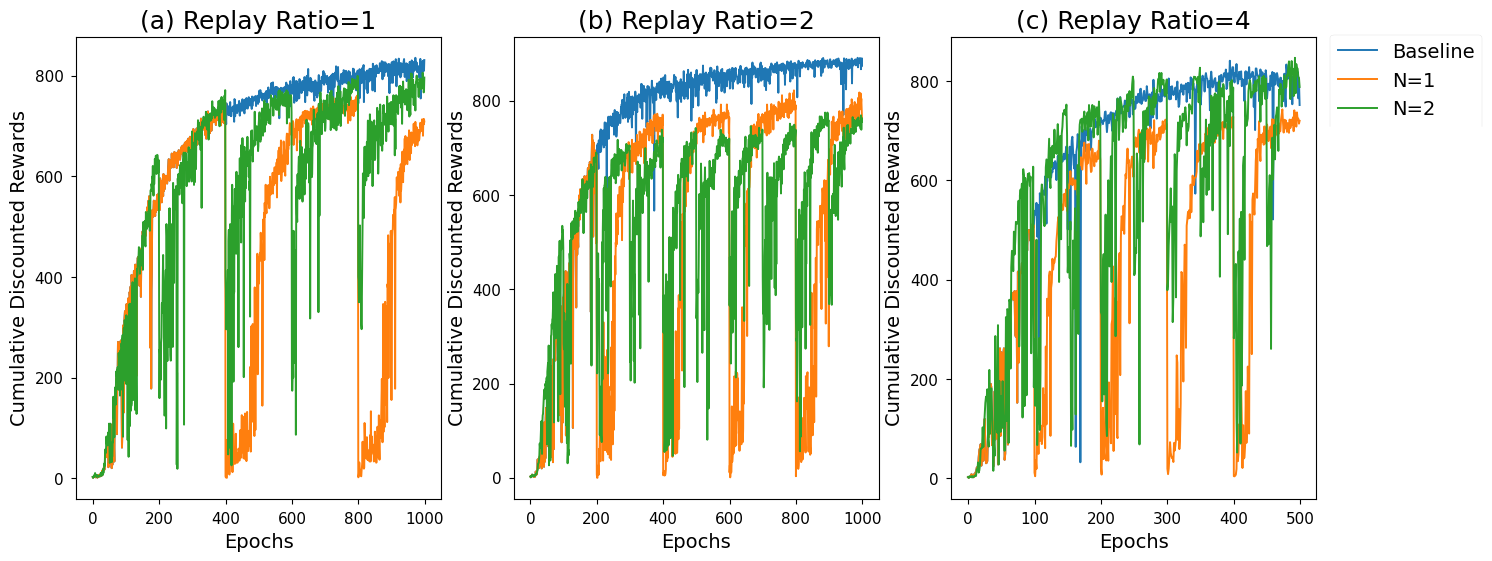
\includegraphics[width = 1 \linewidth]{cheetah_fig.png}
	\begin{flushleft} For \texttt{Cheetah-Run}, this figure displays the performance of the SAC in the baseline case (in blue), with naive resets with one agent (in orange), and with ensemble resets using RDE with two agents (in green). Results are shown across replay ratios of 1, 2, and 4. \end{flushleft}
\end{figure}

From Figure \ref{fig:cheetah}, we can see that when the replay ratio is $1$ or $2$, the baseline SAC algorithm outperforms both the vanilla reset and RDE methods, though not by a very significant margin.
Meanwhile, when the replay ratio is $4$, by the end of the training loop, the RDE method does about as well as the baseline SAC algorithm.
These results are fairly consistent with \cite{kim2023}, who does not observe significant performance improvements from implementing RDE in the \texttt{Cheetah-Run} setting.
However, we note that while our implementation of RDE with SAC does not experience performance collapses as significant as those in the vanilla reset method, they are larger than those observed by \cite{kim2023}.
We identify two reasons for this.
First, given the long training time that is required, we are only able to run our code once, while \cite{kim2023} averages their results over $5$ seeds, so there is some inherent level of randomness that causes our results to differ.
Moreover, given some inconsistencies identified in the discussion that \cite{kim2023} provides on how to tune the $\beta$ parameter in computing $p_{select}$, we believe that this part of our implementation may not exactly match theirs.
Further discussion on this is provided in Section \ref{ssec:errors}.

Next, we display our results in the \texttt{Mountain Car Continuous} setting.
We make comparisons across the baseline SAC algorithm without any agent resets, SAC with naive resets, and SAC with RDE for replay ratios of $1$, $2$, and $4$.
Our results for a replay ratio of $2$ is shown below in Figure \ref{fig:mc_rr2}, while those for replay ratios of $1$ and $4$ can be found in Appendix \ref{app:c}, as we do not find much variation in patterns across the three scenarios.

\begin{figure}[h!]
	\centering
	\caption{Performance Comparison in the \texttt{Mountain Car Continuous} Setting when RR=2}
	\label{fig:mc_rr2}
	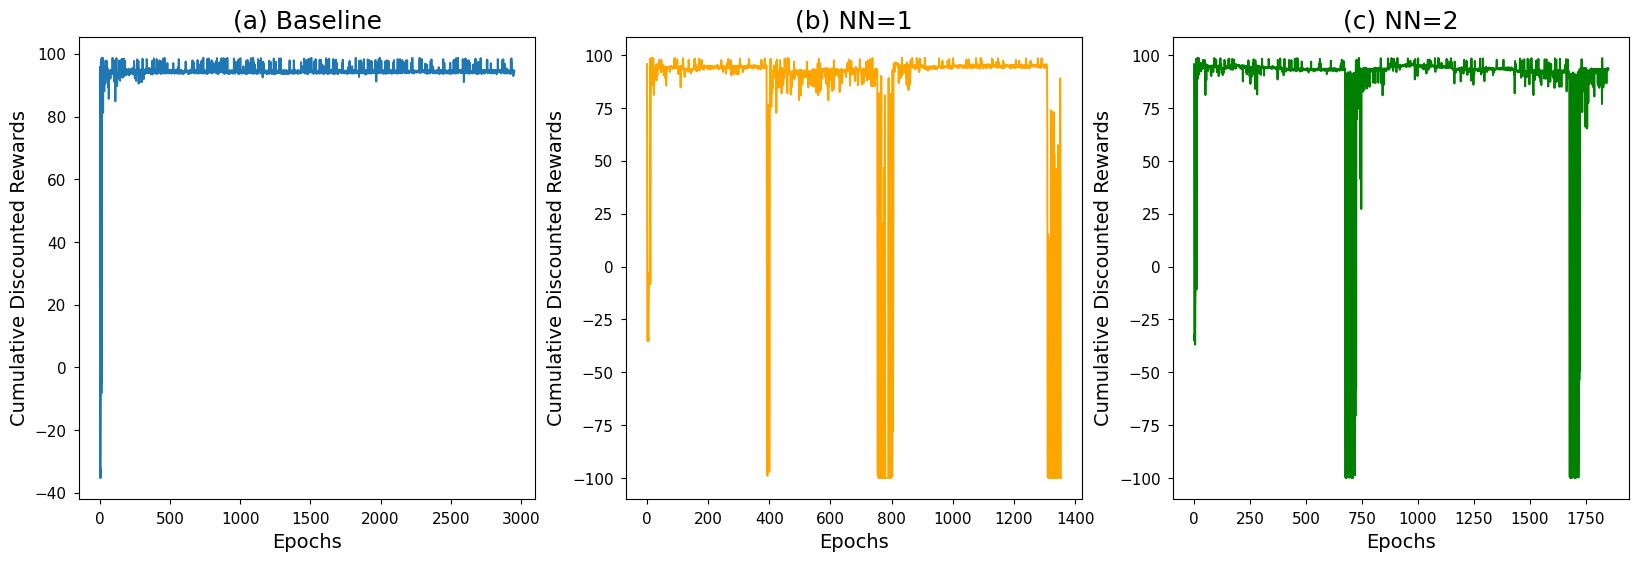
\includegraphics[width = 1 \linewidth]{mc_RR2.png}
	\begin{flushleft} For \texttt{Mountain Car Continuous}, we compare the performance of SAC with a replay ratio of two across the baseline case, with naive resets with one agent, and with ensemble agents using RDE with two agents. \end{flushleft}
\end{figure}

For the \texttt{Mountain Car Continuous} setting, we can see that the baseline SAC algorithm is successful on its own at learning the environment.
This is likely because of the relatively small state and action space of the environment.
Thus, as our algorithm appears to not suffer from primacy bias and overfitting, our results show that agent resets do not bring about significant performance improvements.
Nonetheless, across all three tested replay ratios, we see that performance collapses are more frequent in the naive reset method compared to RDE, demonstrating that RDE is successful in improving safety.
However, we notice that the extent of the drop in rewards experienced in each performance collapse with RDE when $N=2$ is very similar to that in the naive reset method.
Similar to what we observed in the \texttt{Cheetah-Run} environment, we believe that this is the result of our use of the $\beta$ parameter being different than that described by \cite{kim2023}, and we explain this in more detail in Section \ref{ssec:errors}.

Finally, we display results for our simulations in the \texttt{Cart Pole} environment.
Because there is not a significant difference in trends across the three replay ratios we test, we focus on results when the replay ratio is $2$, and these are shown below in Figure \ref{fig:cp_rr2} below.
Meanwhile, results when the replay ratio is $1$ or $4$ are shown in Appendix \ref{app:c}.

\begin{figure}[h!]
	\centering
	\caption{Performance Comparison in the \texttt{Cart Pole} Setting when RR=2}
	\label{fig:cp_rr2}
	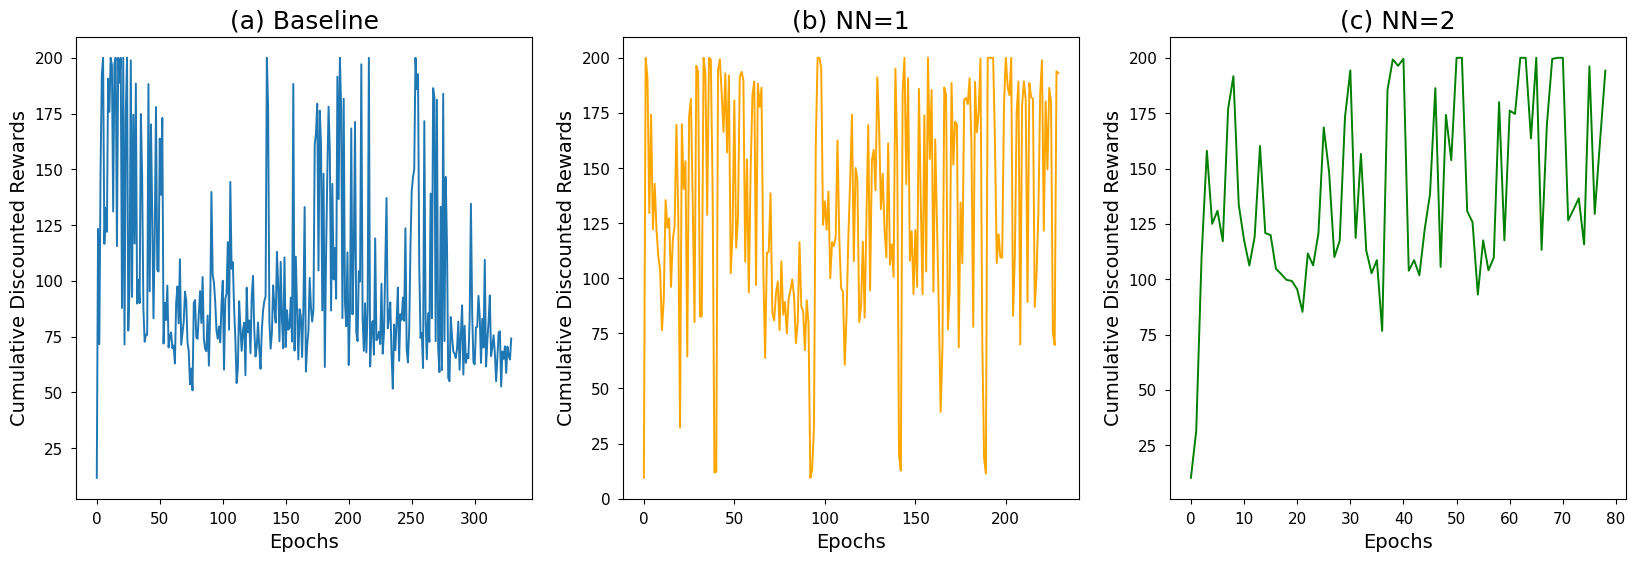
\includegraphics[width = 1 \linewidth]{cp_RR2.png}
	\begin{flushleft} For DQN (using a replay ratio of two) in the baseline case, with naive resets with one agent, and with ensemble agents using RDE with two agents, we display our results. \end{flushleft}
\end{figure}

We observe that the performance collapses observed when using naive resets are significantly greater than those seen when using RDE.
This suggests that RDE indeed does provide a significant improvement over naive resets.
However, because DQN is off-policy, uses bootstrapping, and employs function approximators to describe a large state-action space, it suffers from what is known as the deadly triad \cite{hasselt2018}.
When any of these three components are used together, it has been empirically discovered to be more likely to introduce instabilities to standard RL algorithms, impeding convergence of the optimizer to acceptable policies.
It is also for this reason that it is particularly difficult for DQN to perform well on many of the more complex MiniGrid environments which have sparse rewards, especially when constrained to a short compute time.
The instability of DQN as an algorithm makes it difficult to discern whether some of the performance collapses seen in Figure \ref{fig:cp_rr2} are from noise or agent resets, especially when using RDE.
Nonetheless, because of its added complexity, we note that the RDE algorithm with $N=2$ agents completes a much smaller number of epochs over the same number of training steps as the baseline DQN or naive reset methods, and it is perhaps a direction for future work to evaluate this algorithm over more episode rollouts.

\subsection{Evaluation of the Action Selection Coefficient}
\label{ssec:errors}

We improve upon the results presented by \cite{kim2023} by more thoroughly testing the impact of the action selection coefficient $\beta$, which is used to compute the softmax temperature $\alpha$ in Equation \ref{eq:p_select}.
Here, we notice that there are inconsistencies in their presentation of $\beta$.
Namely, \cite{kim2023} claims that high $\beta$ values yield better performance by adding higher weights to actions chosen by agents that are least recently reset.
While we agree with their assessment that negative values of $\beta$ exacerbate performance collapses, we find that for positive values of $\beta \ge 0$, \textit{lower} $\beta$ values place higher weights on less recently reset agents.
To see this, consider the definition of the softmax function:
for temperature \(\alpha \in \symbb{R}_+\), the softmax function \(s_{\alpha} \colon \symbb{R}^c \to [0,1]^c\) is defined by
\begin{equation*}
	s_{\alpha} \colon x \mapsto \begin{bmatrix}
		\e^{x(1) / \alpha} \\
		\vdots             \\
		\e^{x(c) / \alpha}
	\end{bmatrix} / \sum_{k=1}^c \e^{x(k) / \alpha}.
\end{equation*}

As $\alpha \rightarrow 0$, the sum $\sum_{k=1}^c \e^{x(k) / \alpha}$ gets exponentially larger, hence the softmax function places greater weight on larger input values.
Since $\alpha$ is defined as being directly proportional to $\beta$, the same is true for $\beta$.
This contradicts the statement by \cite{kim2023} that higher $\beta$ values put more weight on actions chosen by less recently reset agents.

To see their claim, \cite{kim2023} tests values of $\beta \in \{-10, 0, 50, 300 \}$.
However, considering $\beta=0$ makes the softmax function in Equation \ref{eq:p_select} undefined from dividing by $0$.
For a replay ratio of one, we run experiments of RDE with TD3 using $N=2$ agents in the \texttt{Cheetah-Run} environment (using the same hyperparameters as those presented in Appendix \ref{app:b} except that we use $2 \times 10^5$ training steps to save time) for varying $\beta$ values in $\{-10, 1, 50, 300\}$.
We plot our results below in Figure \ref{fig:beta_test}, where we observe that $\beta=1$ yields the best performance by placing higher weights on least recently reset agents.
Thus, we believe that the discussion \cite{kim2023} provides on $\beta$ is inconsistent with their definition of $p_{select}$.

\begin{figure}[h!]
	\centering
	\caption{Performance in the \texttt{Cheetah-Run} Setting when RR=1 Across Different $\beta$ Parameter Values}
	\label{fig:beta_test}
	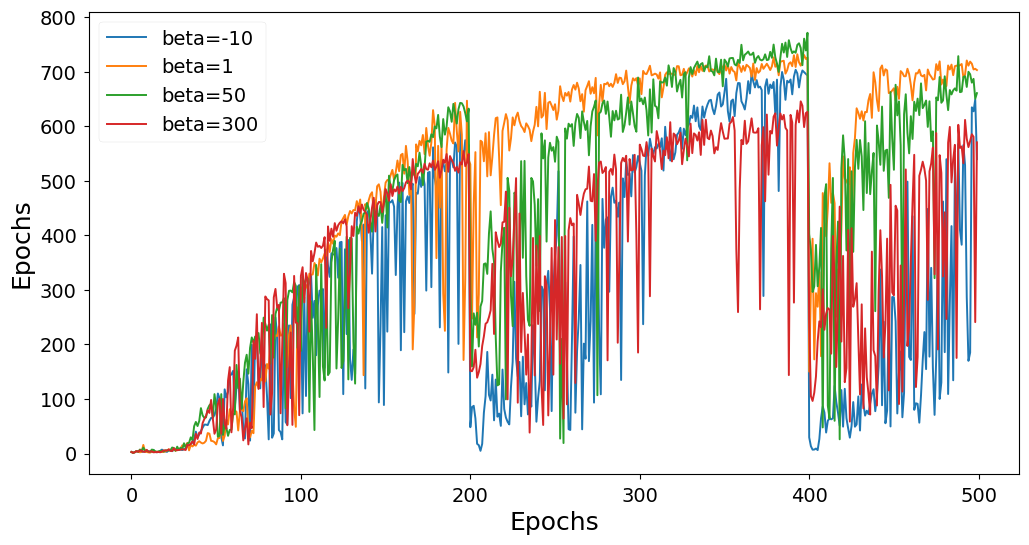
\includegraphics[width = 1 \linewidth]{beta_test.png}
	\begin{flushleft} We display our results of RDE using $N=2$ agents with SAC in the \texttt{Cheetah-Run} setting when the replay ratio is one. We consider $\beta$ parameters in $\{ -10, 1, 50, 300 \}$.  \end{flushleft}
\end{figure}

\section{Conclusion}
\label{sec:conclusion}

In conclusion, by reproducing the results of \cite{kim2023}, we find that RDE indeed does allow for less significant performance collapses, and it is an improvement over the naive reset method proposed by \cite{nikishin2022}.
However, in some cases we have observed that the baseline method with no agent rests performs similarly to the ensemble reset method.
In other environments the baseline stochasticity makes it hard to identify whether performance drops and boosts are due to primacy bias or some other influence such as insufficient duration of training, function approximation errors, or instabilities (e.g. such as those that arise from the deadly triad).
While primacy bias has a precise cause that we can identify, its future effects are usually difficult to identify with confidence, just like primacy bias in cognitive science.
In the sections below, we discuss the limitations of our work and suggest directions for the future.

\subsection{Limitations}
\label{ssec:limits}

The primary limitations in our ability to reproduce the results of \cite{kim2023} are computational power and time.
We list the compute times required for each of our simulations in Appendix \ref{app:d}.
To this end, we could not fully test the entire suite of environments considered in their paper.
Especially for the more complex environments such as Atari-100k and MiniGrid, we did not have the capacity to run a large number of training loops.
As \cite{kim2023} saw varying results across the different environments they considered (including those where RDE significantly outperforms baseline algorithms with no resets), our project is limited in its ability to verify all of their claims.

Moreover, to save time, we also took measures such as using fewer hidden units in our DNNs, taking smaller batches from the replay buffer, taking fewer total training steps, and only running simulations on one seed rather than averaging results over multiple.
Meanwhile, as \cite{kim2023} is inconsistent in their discussion of the $\beta$ parameter, this could also be causing differences in our experimental results.
Thus, we can see that while our results generally align with those found by \cite{kim2023}, differences in implementations do cause some variation in results.

\subsection{Future Work}
\label{ssec:future}

With more time and greater computational resources, there are many directions that can be explored.
For instance, varying parameters such as the replay ratio and the reset interval $T_{reset}$ or resetting only some of the layers of the DNNs being trained are all possible future steps.
In addition, it would be interesting to run simulations with a larger ensemble.
This will allow us to test whether choosing actions based on a larger ensemble of agents will further mitigate primacy bias or if there are diminishing returns after two models.
Similarly, experimenting with different methods of selecting an agent could be worthwhile as well, as there could be better ways to formulate the probability distribution $p_{reset}$ than that in Equation \ref{eq:p_select}.

Furthermore, more simulations across a larger number of seeds can help us better understand the extent to which underlying stochasticity is impacting our observed results.
To this end, further tests over a wider variety of environments that range in difficulty will help validate the results of \cite{kim2023}.
In addition, considering the impacts of RDE on a wider set of algorithms could also prove to be insightful.
As an example, we suggest a possible improvement on temperature annealing in Appendix \ref{app:a}.


\ifSubfilesClassLoaded{%
	\clearpage
	\printbibliography
}{}

\end{document}